\documentclass[journal]{IEEEtran}


% correct bad hyphenation here
\hyphenation{}
\usepackage{amsmath}
\usepackage{comment}
\usepackage{booktabs}
\usepackage{graphicx}
%\usepackage{cases}
%\usepackage{subeqnarray}

\begin{document}
%
% paper title
% Titles are generally capitalized except for words such as a, an, and, as,
% at, but, by, for, in, nor, of, on, or, the, to and up, which are usually
% not capitalized unless they are the first or last word of the title.
% Line-breaks \\ can be used within to get better formatting as desired.
% Do not put math or special symbols in the title.
\title{Saliency Prediction for Children with Autism Spectrum Disorder}


\author{Zhengke~Wu, Jiaqi~Ma, Ruofeng~Liu
\thanks{This work is part of the final project of CS386 Digital Image Processing in SJTU, 2020 Fall.}}

% make the title area
\maketitle

% As a general rule, do not put math, special symbols or citations
% in the abstract or keywords.
\begin{abstract}
Autism spectrum disorder (ASD) is a common neurodevelopmental illnesses for children, which may lead to atypical visual attention and behaviors. Therefore, learning the visual attention of children wit ASD contributes to related research in the field of medicine and psychology. In this work, we propose a saliency prediction model for children with ASD. The backbone of our model is $\text{U}^2$-Net, currently the state-of-the-art method for saliency object detection with deep convolutional neural networks. Then we do transfer learning on a saliency prediction for children with autism (SPCA) database to train and finetune the model. Experiments show that this model can obtain satisfying performance on test data.
\end{abstract}

% Note that keywords are not normally used for peerreview papers.
\begin{IEEEkeywords}
Saliency prediction, visual attention, autism spectrum disorder
\end{IEEEkeywords}

\IEEEpeerreviewmaketitle

\section{Introduction}

As this is just a course project report, we don't think it's necessary to include a lengthy and boring introduction section. 

So that's it. Let's go straight to the point.

\section{Proposed Method}

Basically, we use $\text{U}^2$-Net \cite{Qin_2020_PR} as our model's backbone as it's the state-of-the-art saliency object detection method so far. Then we do transfer learning \cite{pan2009survey} to train and finetune it with custom loss functions we define.

\subsection{Backbone}

\begin{figure*}
    \centering
    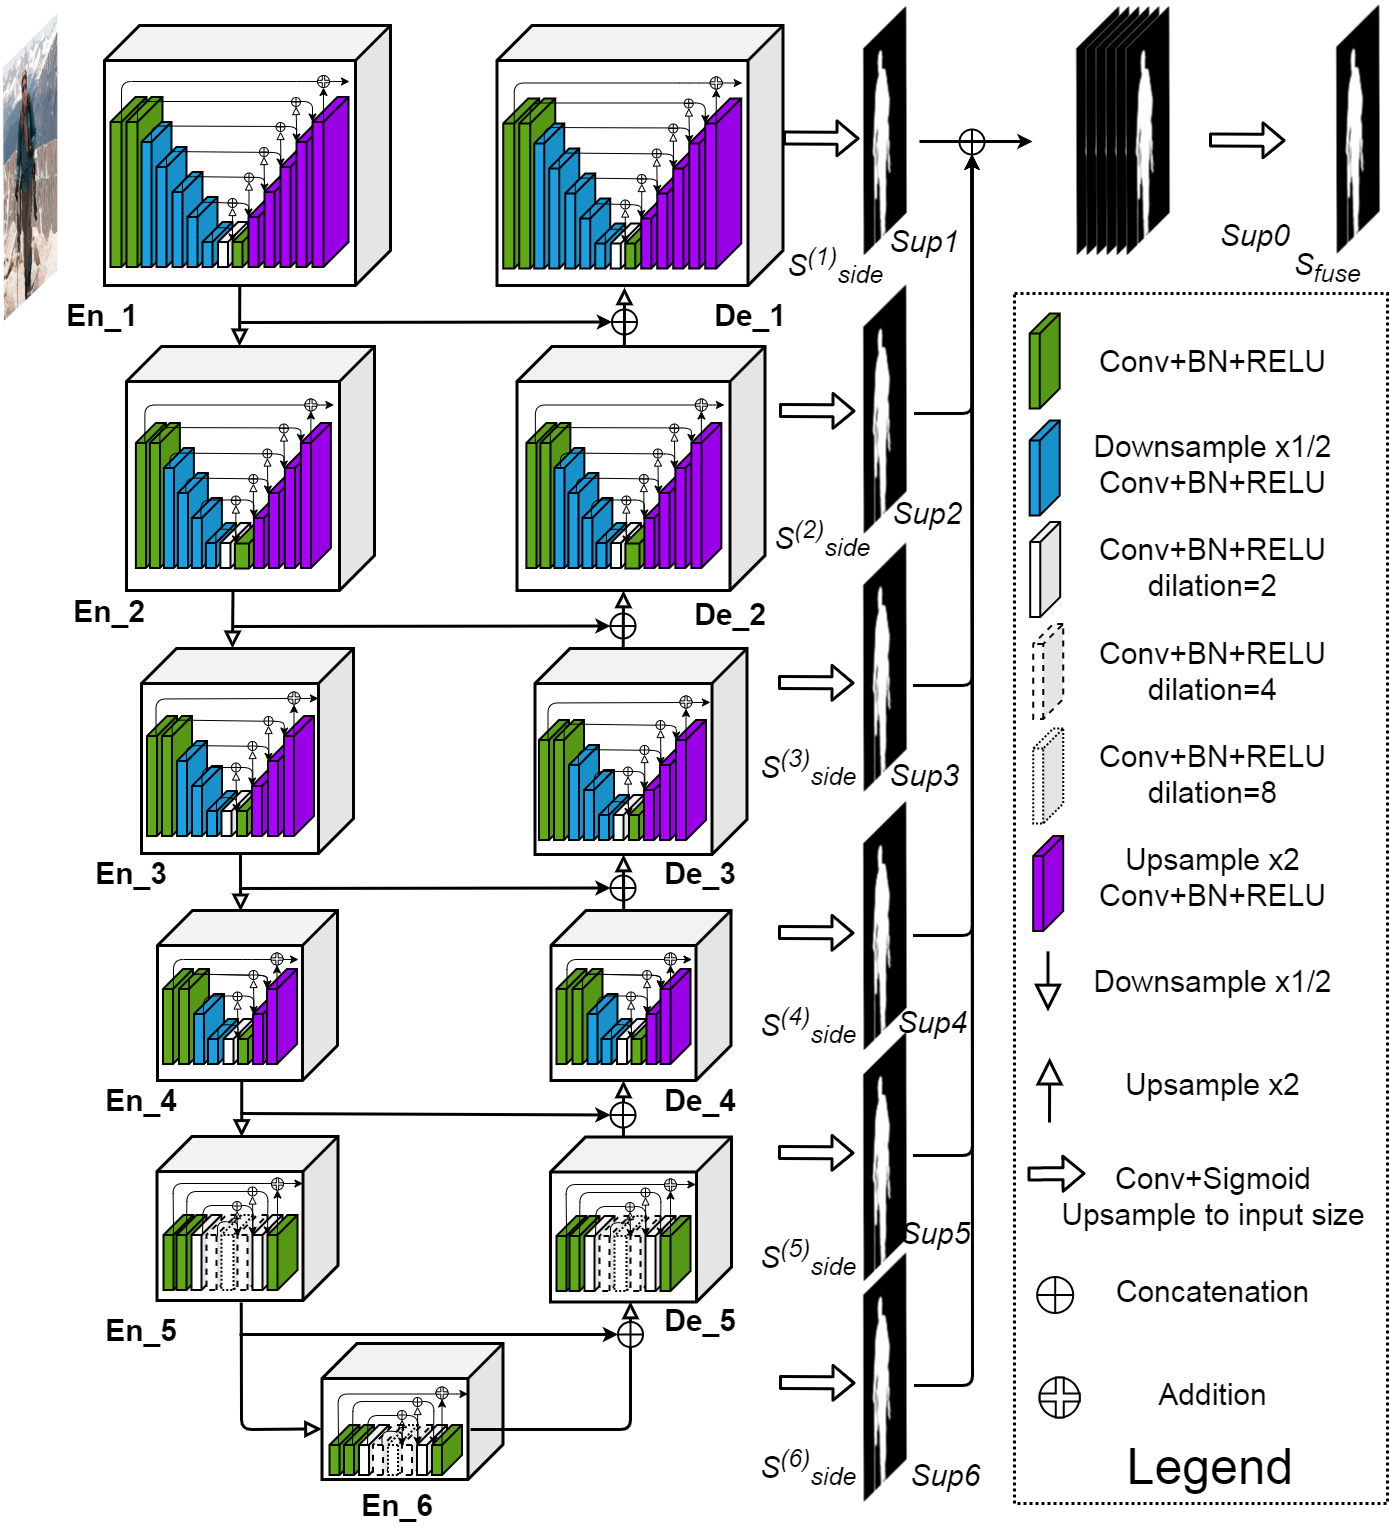
\includegraphics[height=.5\textheight]{u-2-net-architecture.png}
    \caption{The overall architecture of $\text{U}^2$-Net, figure from \cite{Qin_2020_PR}.}
    \label{fig:u-2-net-architecture}
\end{figure*}

For saliency prediction or saliency object detection, there are multiple existing methods like Shallow ConvNet \cite{Pan_2016_CVPR}, ML-Net \cite{mlnet2016}, SalGan \cite{Pan_2017_SalGAN}, BASNet \cite{Qin_2019_CVPR} and $\text{U}^2$-Net \cite{Qin_2020_PR}. They all perform well on regular saliency prediction tasks and data-sets. But as they're not designed for saliency prediction for children with autism spectrum disorder, we need to train and finetune them to make full use of their potential.

Proposed by \textit{Qin et al.} \cite{Qin_2020_PR}, $\text{U}^2$-Net is currently the state-of-the-art solution to saliency object detection. As is shown in Fig. \ref{fig:u-2-net-architecture}, the main architecture of $\text{U}^2$-Net is a big U-structure of 11 stages and each stage is a residual U-block (RSU) \cite{Qin_2020_PR} encoder or decoder. Therefore, it's able to capture rich local and global information from both shallow and deep layers, extract multi-level features from original input images and then fuse these multi-level features together. 

\subsection{Transfer Learning}

As saliency prediction for children with autism spectrum disorder was not a hot topic, we can only obtain a small number of training samples (for example, there are around 300 images in the dataset of eye movements for children with autism spectrum disorder \cite{duan_huiyu_2019_2647418}), which is not enough for us to train a model from scratch without the pain of over-fitting, we decide to do transfer learning.

$\text{U}^2$-Net authors provide a pretrained model\footnote{https://github.com/NathanUA/BASNet} on regular saliency object detection datasets like SOD \cite{newell2016stacked}, ECSSD \cite{yan2013hierarchical}, DUT-OMRON \cite{yang2013saliency}, PASCAL-S \cite{li2014secrets}, HKU-IS \cite{li2016visual} and DUTS-TE \cite{wang2017learning}, which performs excellently for regular saliency object detection. So we use this pretrained model to start our training.

\section{Experiments}

\subsection{Experimental Setup}

We use the dataset of eye movements for children with autism spectrum disorder \cite{duan_huiyu_2019_2647418} to validate the performance of our proposed method. This dataset includes 300 images and for each image it has saliency map, fixation map and other additional information for children with ASD and typical developed children. We divide the dataset into three parts randomly: 70\% for training, 10\% for validation and 20\% for testing.

In the training process, we use binary cross entropy (BCE) to compute loss between predicted saliency map and ground truth saliency map:

\begin{equation}
    \textbf{BCE}_y(p) = -\frac{1}{N}\sum_{i=1}^{N}y_i\log(p_i) + (1 - y_i)\log(1 - p_i)
\end{equation}
where $p$ is the predicted saliency map, $y$ is the ground truth and $N$ is the number of pixels.

Adam \cite{kingma2014adam} with learning rate of 0.001 and no weight decay is used to optimize parameters in each step (consistent with the setup of $\text{U}^2$-Net). 

Our model is trained on a cloud server with one Nvidia Tesla P4 GPU.

\subsection{Experimental Results}

\begin{figure*}
    \centering
    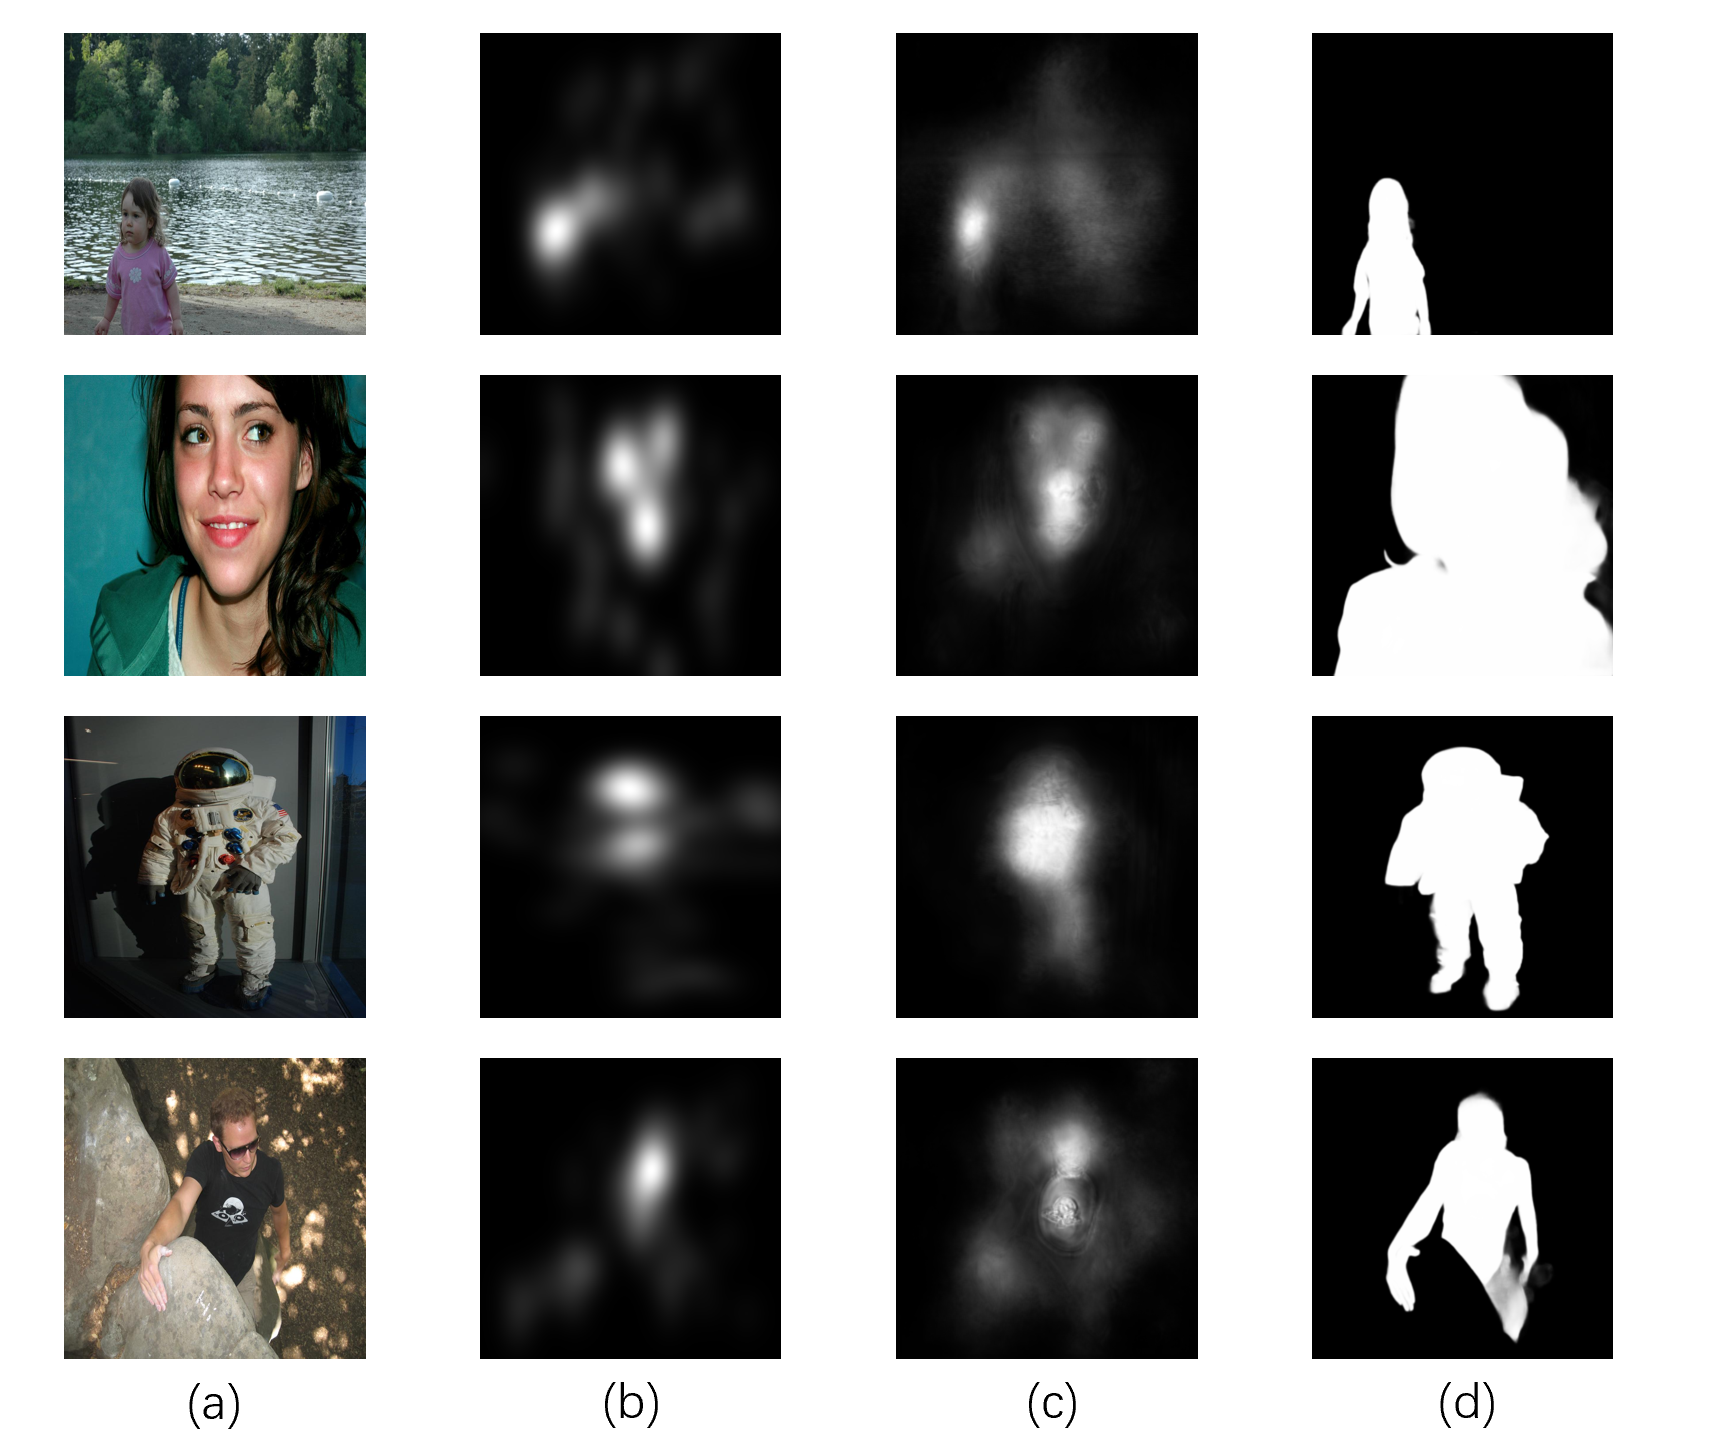
\includegraphics[height=.4\textheight]{examples.png}
    \caption{Saliency maps. From left to right: (a) original images, (b) ground truth (children with ASD), (c) our model's prediction, (d) the pretrained $\text{U}^2$-Net's prediction.}
    \label{fig:examples}
\end{figure*}

First, there are some random-selected examples in Fig. \ref{fig:examples} for us to have a qualitative understanding of our model. We can see that the pretrained $\text{U}^2$-Net performs excellently for regular saliency object detection, and after our transfer learning, it can learn the saliency map for children with ASD pretty well. Also, compared with the ground truth, there are some blurring regions in our prediction, which we think could be addressed with further image processing.

Then we use MIT saliency benchmark \cite{mit-saliency-benchmark}'s code to quantitatively evaluate our model. As suggested by \cite{salMetrics_Bylinskii}, we compute metrics including Pearson Linear Correlation Coefficient (CC), Area Under the ROC Curve (AUC), Normalized Scanpath Saliency (NSS), Kullback-Leibler Divergence (KL) and saliency map similarity (SIM). The results of our model are shown in Table \ref{tab:metrics}. 

\begin{table}[]
\centering
\caption{Evaluation metrics for our model}\label{tab:metrics}
\begin{tabular}{ll}
\toprule
Evaluation Metric & Result \\
\midrule
SIM($\uparrow$)             & 0.673  \\
CC($\uparrow$)                & 0.756  \\
KL($\downarrow$)                & 0.534  \\
NSS($\uparrow$)               & 1.641  \\
AUC-J($\uparrow$)             & 0.354  \\
AUC-B($\uparrow$)            & 0.655 \\
\bottomrule
\end{tabular}
\end{table}

\section{Conclusion}
In this work, we propose a saliency prediction model for children with autism spectrum disorder (ASD). We use $\text{U}^{2}$-Net as its backbone and then do transfer learning on a saliency prediction for children with autism (SPCA) database. We also do some experiments to validate our model's performance. Results confirm that our model can achieve satisfying performance.

\bibliographystyle{IEEEtran}
\bibliography{Ref}


% that's all folks
\end{document}


